%%%%%%%%%%%%%%%%%%%%%%%%%%%%%%%%%%%%%%%%%%%%%%%%%%%%%%%%%%%%
%%% ELIFE ARTICLE TEMPLATE
%%%%%%%%%%%%%%%%%%%%%%%%%%%%%%%%%%%%%%%%%%%%%%%%%%%%%%%%%%%%
%%% PREAMBLE 
\documentclass[9pt,lineno]{elife}

\usepackage[version=4]{mhchem}
\usepackage{siunitx}
\usepackage{makecell}
\usepackage[colorinlistoftodos]{todonotes} % To add todos.
\DeclareSIUnit\Molar{M}

%%%%%%%%%%%%%%%%%%%%%%%%%%%%%%%%%%%%%%%%%%%%%%%%%%%%%%%%%%%%
%%% ARTICLE SETUP
%%%%%%%%%%%%%%%%%%%%%%%%%%%%%%%%%%%%%%%%%%%%%%%%%%%%%%%%%%%%
\title{Binding thermodynamics of host-guest systems with SMIRNOFF99Frosst, an Open Force Field Group product}

\author[1]{David R. Slochower}
\author[2]{Niel M. Henriksen}
% \author[3]{Michael R. Shirts}
\author[5]{John D. Chodera}
% \author[4]{David L. Mobley}
\author[1]{Michael K. Gilson}

\affil[1]{Skaggs School of Pharmacy and Pharmaceutical Sciences, University of California, San Diego, La Jolla, CA 92093, USA}
\affil[2]{Atomwise, Inc., San Francisco, CA 94105, USA}
% \affil[3]{Department of Chemical and Biological Engineering, University of Colorado Boulder, Boulder, CO 80309}
% \affil[4]{Department of Pharmaceutical Sciences and Department of Chemistry, University of California, Irvine, CA 92697, USA}
\affil[5]{Computational and Systems Biology Program, Sloan Kettering Institute, Memorial Sloan Kettering Cancer Center, New York, NY 10065}

\corr{mgilson@ucsd.edu}{MKG}

\newif\ifdraft
\drafttrue
\ifdraft
 \newcommand{\drsnote}[1]{ {\textcolor{red} { [DRS: #1] }}}
\else
 \newcommand{\drsnote}[1]{}
\fi


%%%%%%%%%%%%%%%%%%%%%%%%%%%%%%%%%%%%%%%%%%%%%%%%%%%%%%%%%%%%
%%% ARTICLE START
%%%%%%%%%%%%%%%%%%%%%%%%%%%%%%%%%%%%%%%%%%%%%%%%%%%%%%%%%%%%

\begin{document}

\maketitle
\drsnote{I have only included authors who reviewed the outline; I'm willing to revisit this issue in the future.}

\begin{abstract}

\end{abstract}

\section{Introduction}

\section{Methods}
\subsection{Host-guest systems}

In this manuscript, we report the binding thermodynamics for 43 host-guest complexes which were experimentally characterized in \cite{rekharsky_thermodynamic_1997} and previously studied in \cite{henriksen_evaluating_2017}. The host molecules are $\alpha$- or $\beta$-cyclodextrin with guests that can be characterized by their functional group as either ammonium, carboxylate, or cyclic alcohol. As before, only one stereoisomer was considered by the 1-methylammonium guests as it was unclear from the experimental details whether a mixture was used, and if so, what ratio was used.

To aid in benchmarking, we used exactly the same hosts and guests as our previous study.

\subsection{Force field parameters}
Host-guest systems were parameterized with 



GAFF v1.7 from Niel
GAFF v2.1 from AMBER18.


A single glucose molecule with methoxy caps on the O1 and O4 alcohols... AM1-BCC partial charges and GAFF v.17 Lennard-Jones and valence parameters.

GAFF v2.1 

\subsection{Simulations}
GAFF v1.7 simulations were performed with AMBER16; GAFF v2.1 and SMIRNOFF99Frosst simulations were performed with AMBER18 molecular dynamics software.

- 2000 or 2210 waters.


The coordinates were ketp the same, but force field parameters were converted via this package.


These calculations were performed with the Open Force Field Toolkit to version 0.0.3 and SMRINOFF99Frosst version 1.0.5.


\subsection{Thermodynamic calculations}
We used the attach-pull-release (APR) method as implemented in the open source package pAPRika, version 0.0.3.

A complete description of the APR method is described in \cite{henriksen_computational_2015}.

\section{Results}
SMIRNOFF99Frosst does as well as GAFF, despite far fewer numerical force field parameters.


\begin{figure}[tb]
\centering
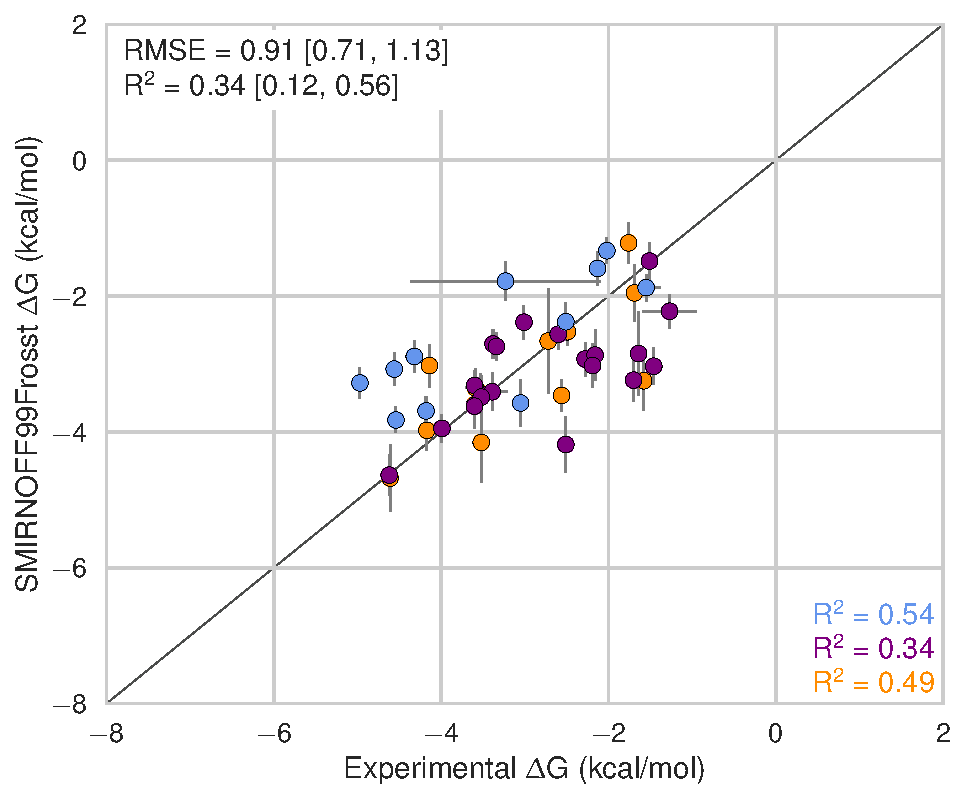
\includegraphics[width=0.49\textwidth]{images/SMIRNOFF99Frosst-vs-Experiment-dG.pdf}
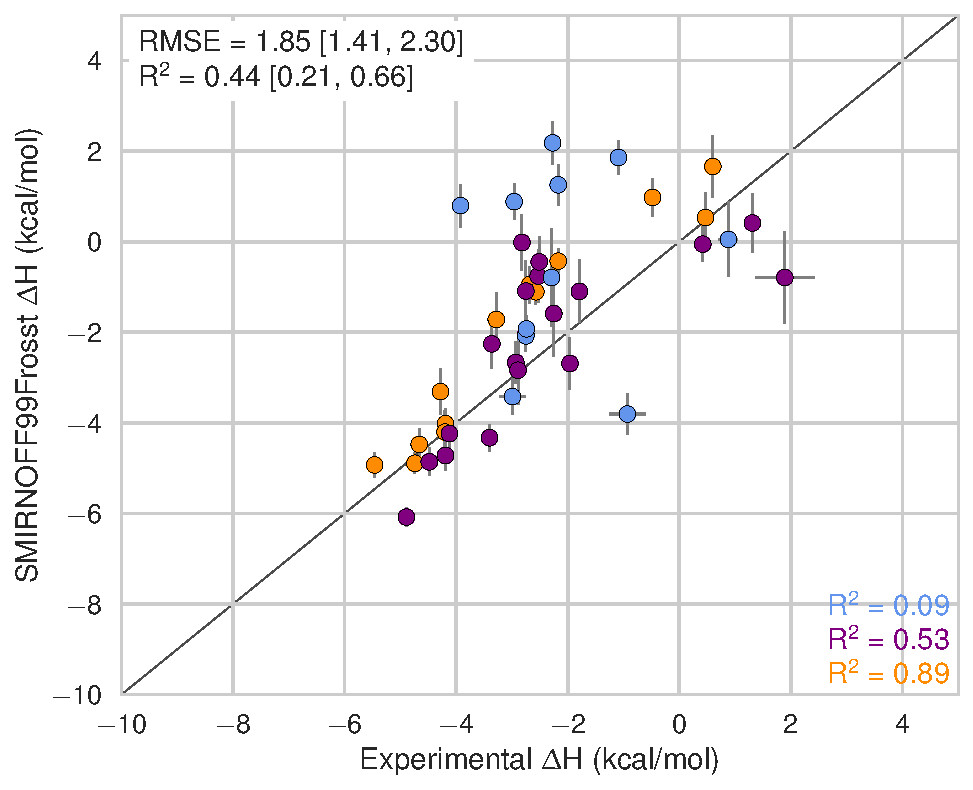
\includegraphics[width=0.49\textwidth]{images/SMIRNOFF99Frosst-vs-Experiment-dH.pdf}
\caption{Caption}
\label{fig:S99-vs-experiment}
\end{figure}

\begin{figure}[tb]
\centering
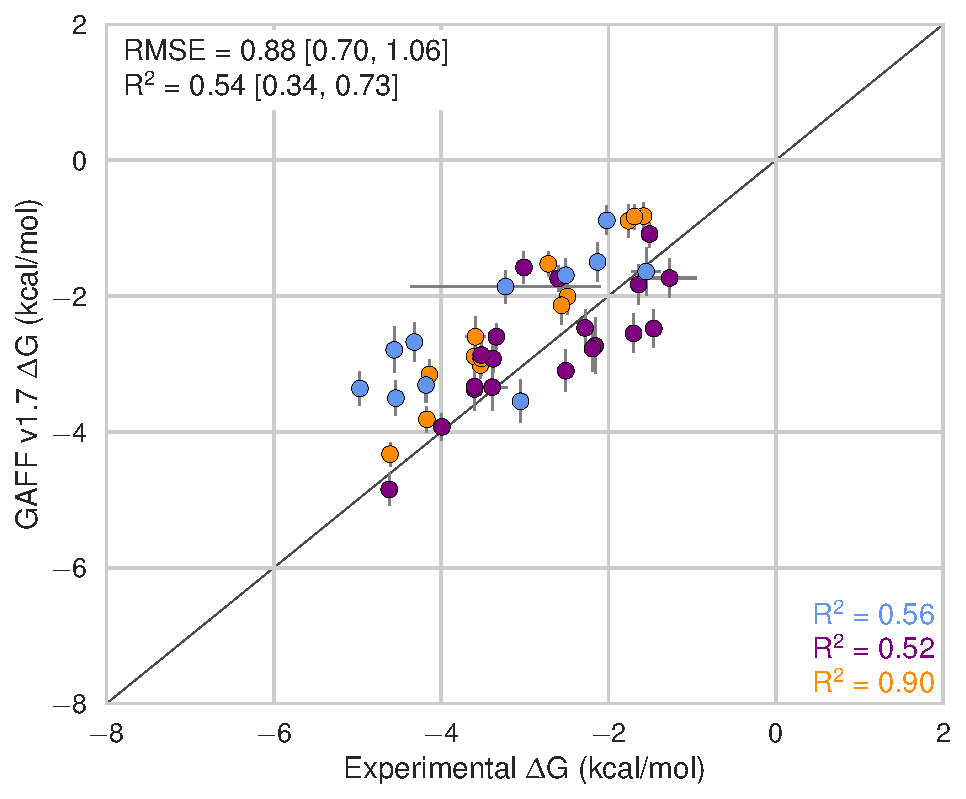
\includegraphics[width=0.49\textwidth]{{images/GAFF-v1.7-vs-Experiment-dG}.pdf}
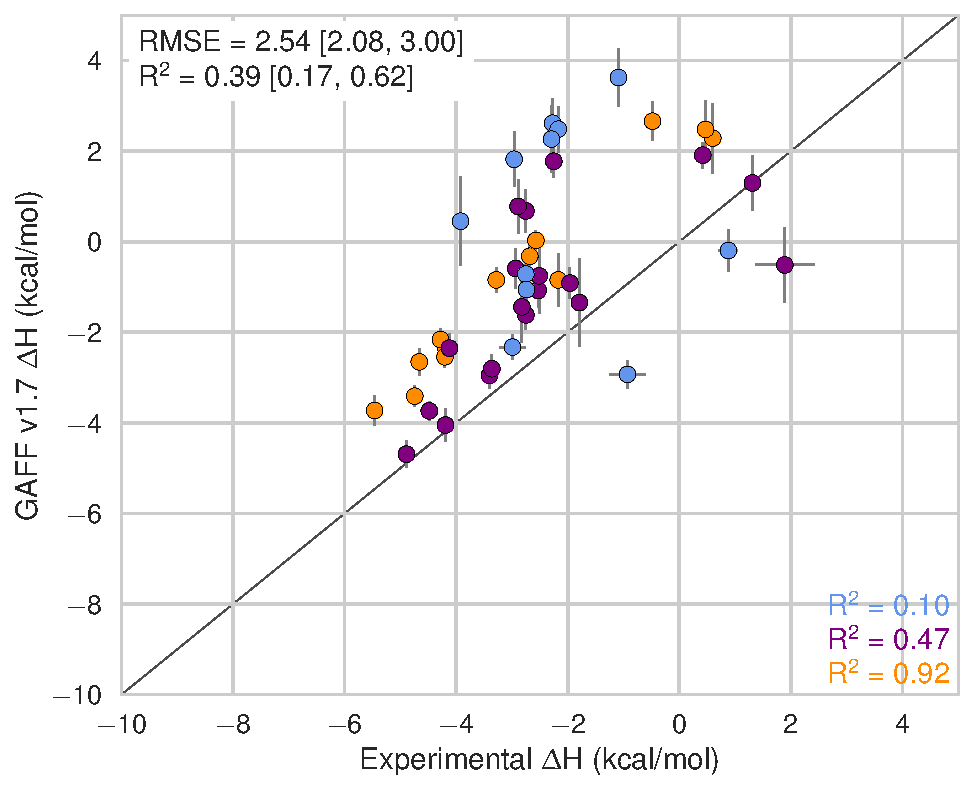
\includegraphics[width=0.49\textwidth]{{images/GAFF-v1.7-vs-Experiment-dH}.pdf}
\caption{Caption}
\label{fig:GAFF-v17-vs-experiment}
\end{figure}

\begin{figure}[tb]
\centering
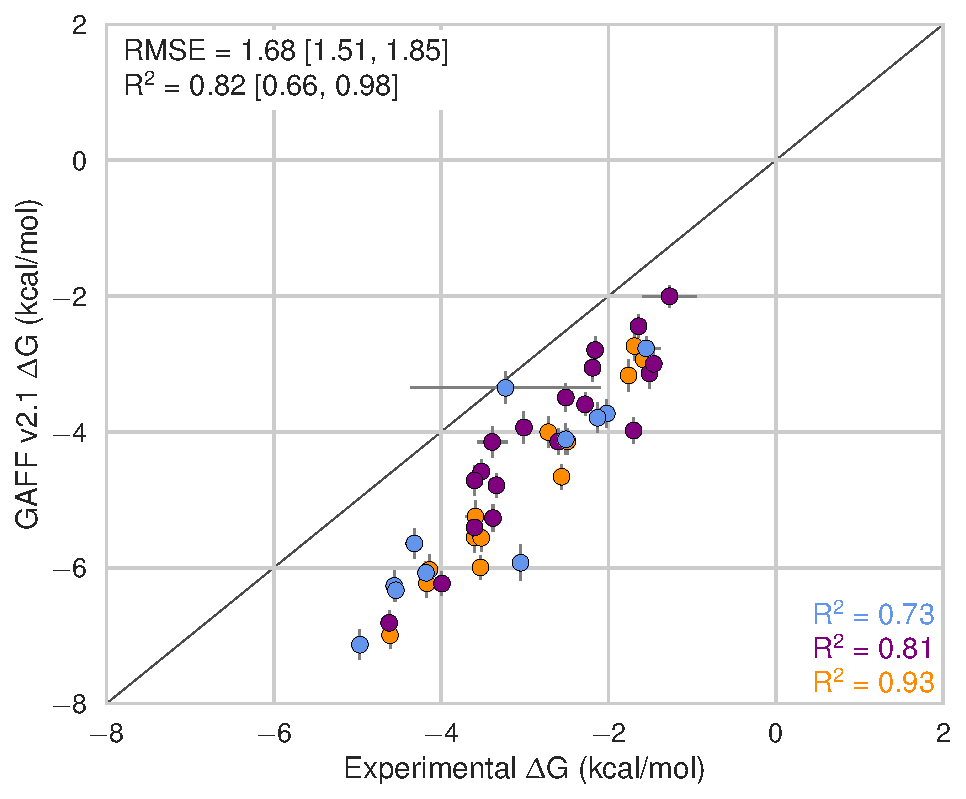
\includegraphics[width=0.49\textwidth]{{images/GAFF-v2.1-vs-Experiment-dG}.pdf}
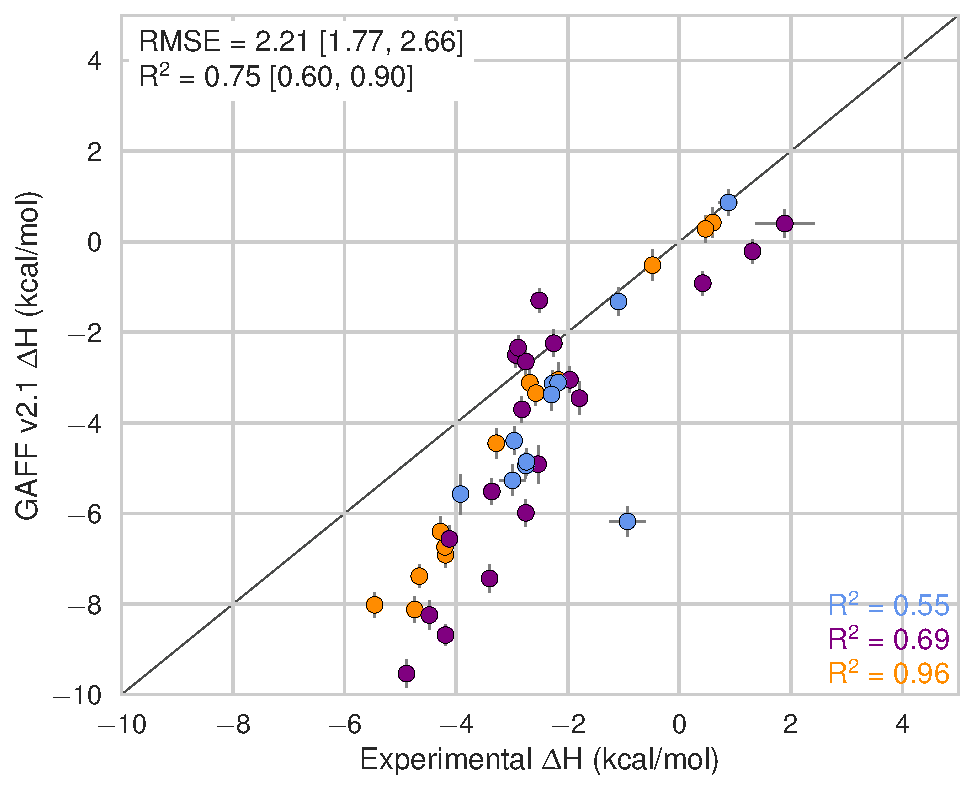
\includegraphics[width=0.49\textwidth]{{images/GAFF-v2.1-vs-Experiment-dH}.pdf}
\caption{Caption}
\label{fig:GAFF-v21-vs-experiment}
\end{figure}

\section{Discussion}

%%%%%%%%%%%%%%%%%%%%%%%%%%%%%%%%%%%%%%%%%%%%%%%%%%%%%%%%%%%%%%%%%%%%%%%%%%%%%%%%%%%%%%%%%%%%%%%%%%%%%%
% Code and Data Availability
%%%%%%%%%%%%%%%%%%%%%%%%%%%%%%%%%%%%%%%%%%%%%%%%%%%%%%%%%%%%%%%%%%%%%%%%%%%%%%%%%%%%%%%%%%%%%%%%%%%%%%

\section{Code and data availability}

%%%%%%%%%%%%%%%%%%%%%%%%%%%%%%%%%%%%%%%%%%%%%%%%%%%%%%%%%%%%%%%%%%%%%%%%%%%%%%%%%%%%%%%%%%%%%%%%%%%%%%
% Author Contributions 
%%%%%%%%%%%%%%%%%%%%%%%%%%%%%%%%%%%%%%%%%%%%%%%%%%%%%%%%%%%%%%%%%%%%%%%%%%%%%%%%%%%%%%%%%%%%%%%%%%%%%%
\section{Author Contributions}
Conceptualization, DRS, NMH, JDC, MKG; Methodology, DRS, NMH; Software, DRS, NMH; Formal Analysis, DRS, NMH, JDC, MKG; Investigation, DRS, NMH; Resources, MKG, JDC;  Data Curation, DRS, NMH; Writing-Original Draft, DRS, NMH; Writing - Review and Editing, DRS, NMH, JDC, MKG; Visualization, DRS; Supervision, JDC, MKG; Project Administration, MKG; Funding Acquisition, MKG.

%%%%%%%%%%%%%%%%%%%%%%%%%%%%%%%%%%%%%%%%%%%%%%%%%%%%%%%%%%%%%%%%%%%%%%%%%%%%%%%%%%%%%%%%%%%%%%%%%%%%%%
% Acknowledgments 
%%%%%%%%%%%%%%%%%%%%%%%%%%%%%%%%%%%%%%%%%%%%%%%%%%%%%%%%%%%%%%%%%%%%%%%%%%%%%%%%%%%%%%%%%%%%%%%%%%%%%%
\section{Acknowledgments}
The authors declare the following competing financial interest(s): MKG has an equity interest in and is a cofounder and scientific advisor of VeraChem LLC.
%%%%%%%%%%%%%%%%%%%%%%%%%%%%%%%%%%%%%%%%%%%%%%%%%%%%%%%%%%%%%%%%%%%%%%%%%%%%%%%%%%%%%%%%%%%%%%%%%%%%%%
% Disclosures 
%%%%%%%%%%%%%%%%%%%%%%%%%%%%%%%%%%%%%%%%%%%%%%%%%%%%%%%%%%%%%%%%%%%%%%%%%%%%%%%%%%%%%%%%%%%%%%%%%%%%%%
\section{Disclosures}

\bibliography{references}

%%%%%%%%%%%%%%%%%%%%%%%%%%%%%%%%%%%%%%%%%%%%%%%%%%%%%%%%%%%%
%%% APPENDICES
%%%%%%%%%%%%%%%%%%%%%%%%%%%%%%%%%%%%%%%%%%%%%%%%%%%%%%%%%%%%

\appendix
\section{List of abbreviations}
APR, attach-pull-release
\end{document}
